\section{Method}\label{sec: method}

The method for calibration considers the frames of the accelerometer and gyroscope as two non-orthogonal and misaligned frames, as illustrated in Figure \ref{fig:axis}, and estimates a linear transformation from each sensor's frame to a common orthogonal one.

\begin{figure}[h]
	\centering
	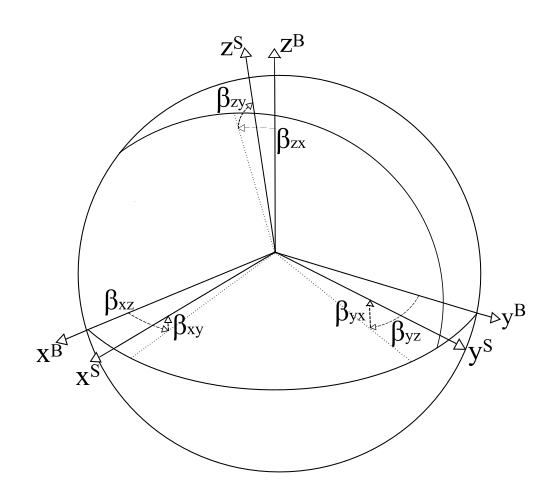
\includegraphics[width=0.5\linewidth]{figures/axis}
	\caption{Accelerometer and Gyroscope axis are non orthogonal and misaligned.}
	\label{fig:axis}
	\source{Reproduced from \cite{2014:Tedaldi}.}
\end{figure}

In other words, let $acc$ and $gyr$ be the accelerometer and gyroscope readings, the method estimates the scale $K_{3\times 3}$, the skew $S_{3\times 3}$ , and the bias $B_{3\times 1}$ for both sensors, and the calibrated measures $acc^*$ and $gyr^*$  are computed as follows:

\begin{equation}
\begin{aligned}
acc^* = K^aS^a(acc - B^a) \\ 
gyr^* = K^gS^g(gyr - B^g) 
\end{aligned}
\end{equation}

\begin{important}
	\begin{enumerate}
		\item The $acc$ and $gyr$ readings given by the IMU are usually in their own scale. The conversion to S.I. is made intrinsically through the scale matrices $S^a$ and $S^g$.
		\item The scale  $K$ is a diagonal matrix (only the $3$ diagonal elements are non-zero),  $S^a$ is a triangle upper matrix ( only the $3$ elements on the upper triangle are non-zero), and $S^g$ is a triangle upper and lower matrix (all the $6$ non-diagonal elements are non-zero).
	\end{enumerate}
\end{important}

The first step is to calculate the calibration parameters for the accelerometer, which is done by optimizing:

\begin{equation}\label{eq: acc opt}
	\argmin_{K^a, S^a, B^a} (||g|| - ||K^aS^a(acc - B^a)||)^2
\end{equation}

Where $g$ is the local gravity, and the $acc$ measures used here belong to the static intervals of the data, which are automatically detected by the tool (more in Section \ref{sec: data collection}).

After the accelerometer is calibrated, the gyroscope is calibrated in two steps.

First, $B^g$ is estimated by averaging the gyroscope measures in the initial static interval (see Section \ref{sec: data collection}).
%
Second, $K^g$ and $S^g$ are estimated by optimizing:

\begin{equation}\label{eq: gyr opt}
	\argmin_{K^g, S^g} \left\|(\tilde{g}_{t_{i+1}}-\tilde{g}_{t_i}) - \int_{t_i}^{t_{i+1}} K^gS^g(gyr - B^g)dt\right\|
\end{equation}

Where $\tilde{g}_{t_i}$ is the gravity versor at time $t_i$, meaning that the term $||\tilde{g}_{t_{i+1}}-\tilde{g}_{t_i})||$ is the angular displacement between to consecutive static intervals, and the integral calculates the angular displacement from the gyroscope readings.

\textbf{Important:}
\begin{important}
	Errors in the accelerometer's calibration will propagate to the gyroscope's calibration giver the later depend on the earlier. 
\end{important}
